\documentclass[submit,techrep]{ipsj_v2/UTF8/ipsj}

\usepackage{latexsym}
\usepackage[dvipdfmx]{graphicx}
\usepackage{amssymb}
\usepackage{enumerate,cite,url}
\usepackage{fancyhdr}
\usepackage{multirow}
\usepackage{threeparttable}
\usepackage{array}
\usepackage{color}
\usepackage{nidanfloat}
\usepackage{setspace}

\pagestyle{fancy}
\renewcommand{\headrulewidth}{0pt} % ヘッダーの羅線をなくす
\lhead[]{\vspace{+2.0cm} \huge A-02}
\chead[]{}
\rhead[]{2017 年度情報処理学会関西支部 支部大会 \\ \ \\}
\cfoot[]{}

\begin{document}

\title{
    {\Huge NoCベース組込みメニーコアでのスケーラブルなデータ配置と並列化}
  \\{\huge Scalable Data Allocation and Parallel Computing \\ on NoC-based Embedded Many Cores}
}

\etitle{\vspace{-3.5cm}}
% \etitle{Componentized Dynamic Memory Allocator for Embedded Systems}

\affiliate{OU}{大阪大学大学院基礎工学研究科\\
Graduate School of Engineering Science, Osaka University}

\affiliate{UT}{東京大学大学院情報理工学系研究科\\
Graduate School of Information Science and Technology, The University of Tokyo}

\author{ {\LARGE 丸山 雄也}}{{\Large Yuya Maruyama}}{OU}%[joho.taro@ipsj.or.jp]
\author{  {\LARGE 加藤 真平}}{{\Large Shinpei Kato}}{UT}%
\author{  {\LARGE 安積 卓也}}{{\Large Takuya Azumi}}{OU}%[gakkai.jiro@ipsj.or.jp]

\maketitle

\pagestyle{empty} \thispagestyle{fancy}

\section{はじめに}
近年,自動車業界をはじめとするいくつかの領域では,高い処理要求と低電力消費を同時に実現するため,マルチ/メニーコアに向けたコンピューティングプラットフォームの進化が求められている \cite{becker2016contention} \cite{faragardi2014communication} \cite{perret2016mapping}.
% この傾向は処理要件が高い組込みシステムにも見られる.
例えば,自動運転システムは様々なアプリケーションを含んでおり,高性能コンピューティングにも分類される.
自動運転システムの高い処理要求,予測可能性,エネルギー効率の要件を考慮すると,マルチ/メニーコアやGPU等のヘテロジニアスなコンピューティングシステムが必要である.
% 低消費電力で高性能な汎用計算を同時に実現するためには,,組込みシステムにおけるマルチ/メニーコアアーキテクチャは重要なトレンドといえる.

しかし,マルチ/メニーコアプラットフォームを組込みシステムに適用するにはいくつかの問題が存在する \cite{becker2016contention} \cite{saidi2015shift}.
例えば,並列化されたプロセス同士で頻繁にアクセス競合が発生する問題や,共有資源が予測可能なタイミング動作やソフトウェア分析を妨げること等が挙げられる.
これらの問題は,組込みシステム特有の厳格な要求仕様や多くのコアによって資源(例えば,メモリ及びI/Oデバイス)を共有することに起因している.
さらに,大容量メモリとすべてのコアを広帯域バスで接続してしまうことで,バス競合によってコア数の拡張性が失われ,大きな電力消費が必要なってしまう問題も存在する.
このコア数の拡張や消費電力の問題に対応するために,Kalrayによって開発されたMulti-Purpose Processing Array (MPPA) -256では,ネットワークオンチップ(NoC)を使用したNUMA(Non-Uniform Memory Access)を採用しており,256のコアと低消費電力を実現している.

組込み要件を考慮すると,コアの数の拡張と妥当な電力効率のためには,マルチ/メニーコアにはNUMAが必要と考えられる.
NUMAによるスケーラブルなデータ割り当てにより,低消費電力で並列化された高性能及び汎用コンピューティングが実現可能である.
MPPA-256は,市販の組込みシステム向けマルチ/メニーコアコンポーネントの1つであり,NoCを用いた分散メモリアーキテクチャを採用している. 
しかし,NoCによる分散メモリ間のデータ転送や並列化の可能性,及びメモリアクセス特性については,アプリケーション開発者には完全には明らかにされていない.
本研究では,上記の項目の定量的評価と組込み向けNoCベースメニーコアプラットフォームの実アプリケーションへの適用を取り上げる.

\textbf{貢献:}
本研究では,MPPA-256等のNoCに基づく組込みのメニーコアコンピューティングの検証に重点を置く.
主に,行列計算によるマイクロベンチマーク評価や自動運転システムの中核をなす自己位置推定アルゴリズムを並列化することにより,下記の2つの貢献を導き,組込み向けメニーコアコンピューティングの実用性と今後の課題を明らかにする.

\begin{itemize}
\item NoCベースのメニーコアプロセッサにおける並列化のスケーラビリティを,様々な状況での行列計算の評価と実際の複雑なアプリケーションの並列化により明らかにする
\item メモリアクセス速度の特性が,データの割り当て先やメモリアクセスの主体によってどのように変化するかを定量的に明らかにする
\end{itemize}

% われわれが知る限り,これは,システム設計者が適切なデータ転送方法を選択できるようにする直感的な予測以上に,多くのコアコンピューティングのデータ転送とデータ割り当ての問題を検証する最初の作業です.
% さらに,自動運転アプリケーションのスピードアップ結果は,NoCベースのマルチコアコンピューティングの実用性を示しています.

\textbf{構成:}
本論文は,以下のように構成される.
まず,本論文で想定するシステムモデルについて\ref{sec:system_model}章で説明する.
ここでは,Kalray MPPA-256 Bostanのハードウェアモデルとソフトウェアモデルを提示する.
次に,\ref{sec:evaluations}章では,評価実験の構成やアプローチについて説明し,評価内容の考察を行う.
続いて,\ref{sec:related_work}章では,マルチ/メニーコアシステムに焦点を当てた関連研究について議論する.
最後に,\ref{sec:conclusion}章にて,まとめとして今後の課題と結論を示す.

\section{システムモデル}
\label{sec:system_model}
本章では,評価に使用されるKalray MPPA-256 Bostanのシステムモデルを示す.
まず,\ref{sec:hardware_model}節にてハードウェアモデルを紹介し,その後に\ref{sec:software_model}節のソフトウェアモデルの説明が続く.

\subsection{ハードウェアモデル}
\label{sec:hardware_model}
MPPA-256プロセッサは,16個のコンピュートクラスタ(CC)及び4個のI/Oサブシステム(IOS)で構成され,これらは全てトーラス状のネットワークオンチップ(NoC)によって接続されている(図\ref{fig:mppa_architecture}と図\ref{fig:noc_map}参照).

\begin{figure}[t]
  \centering
  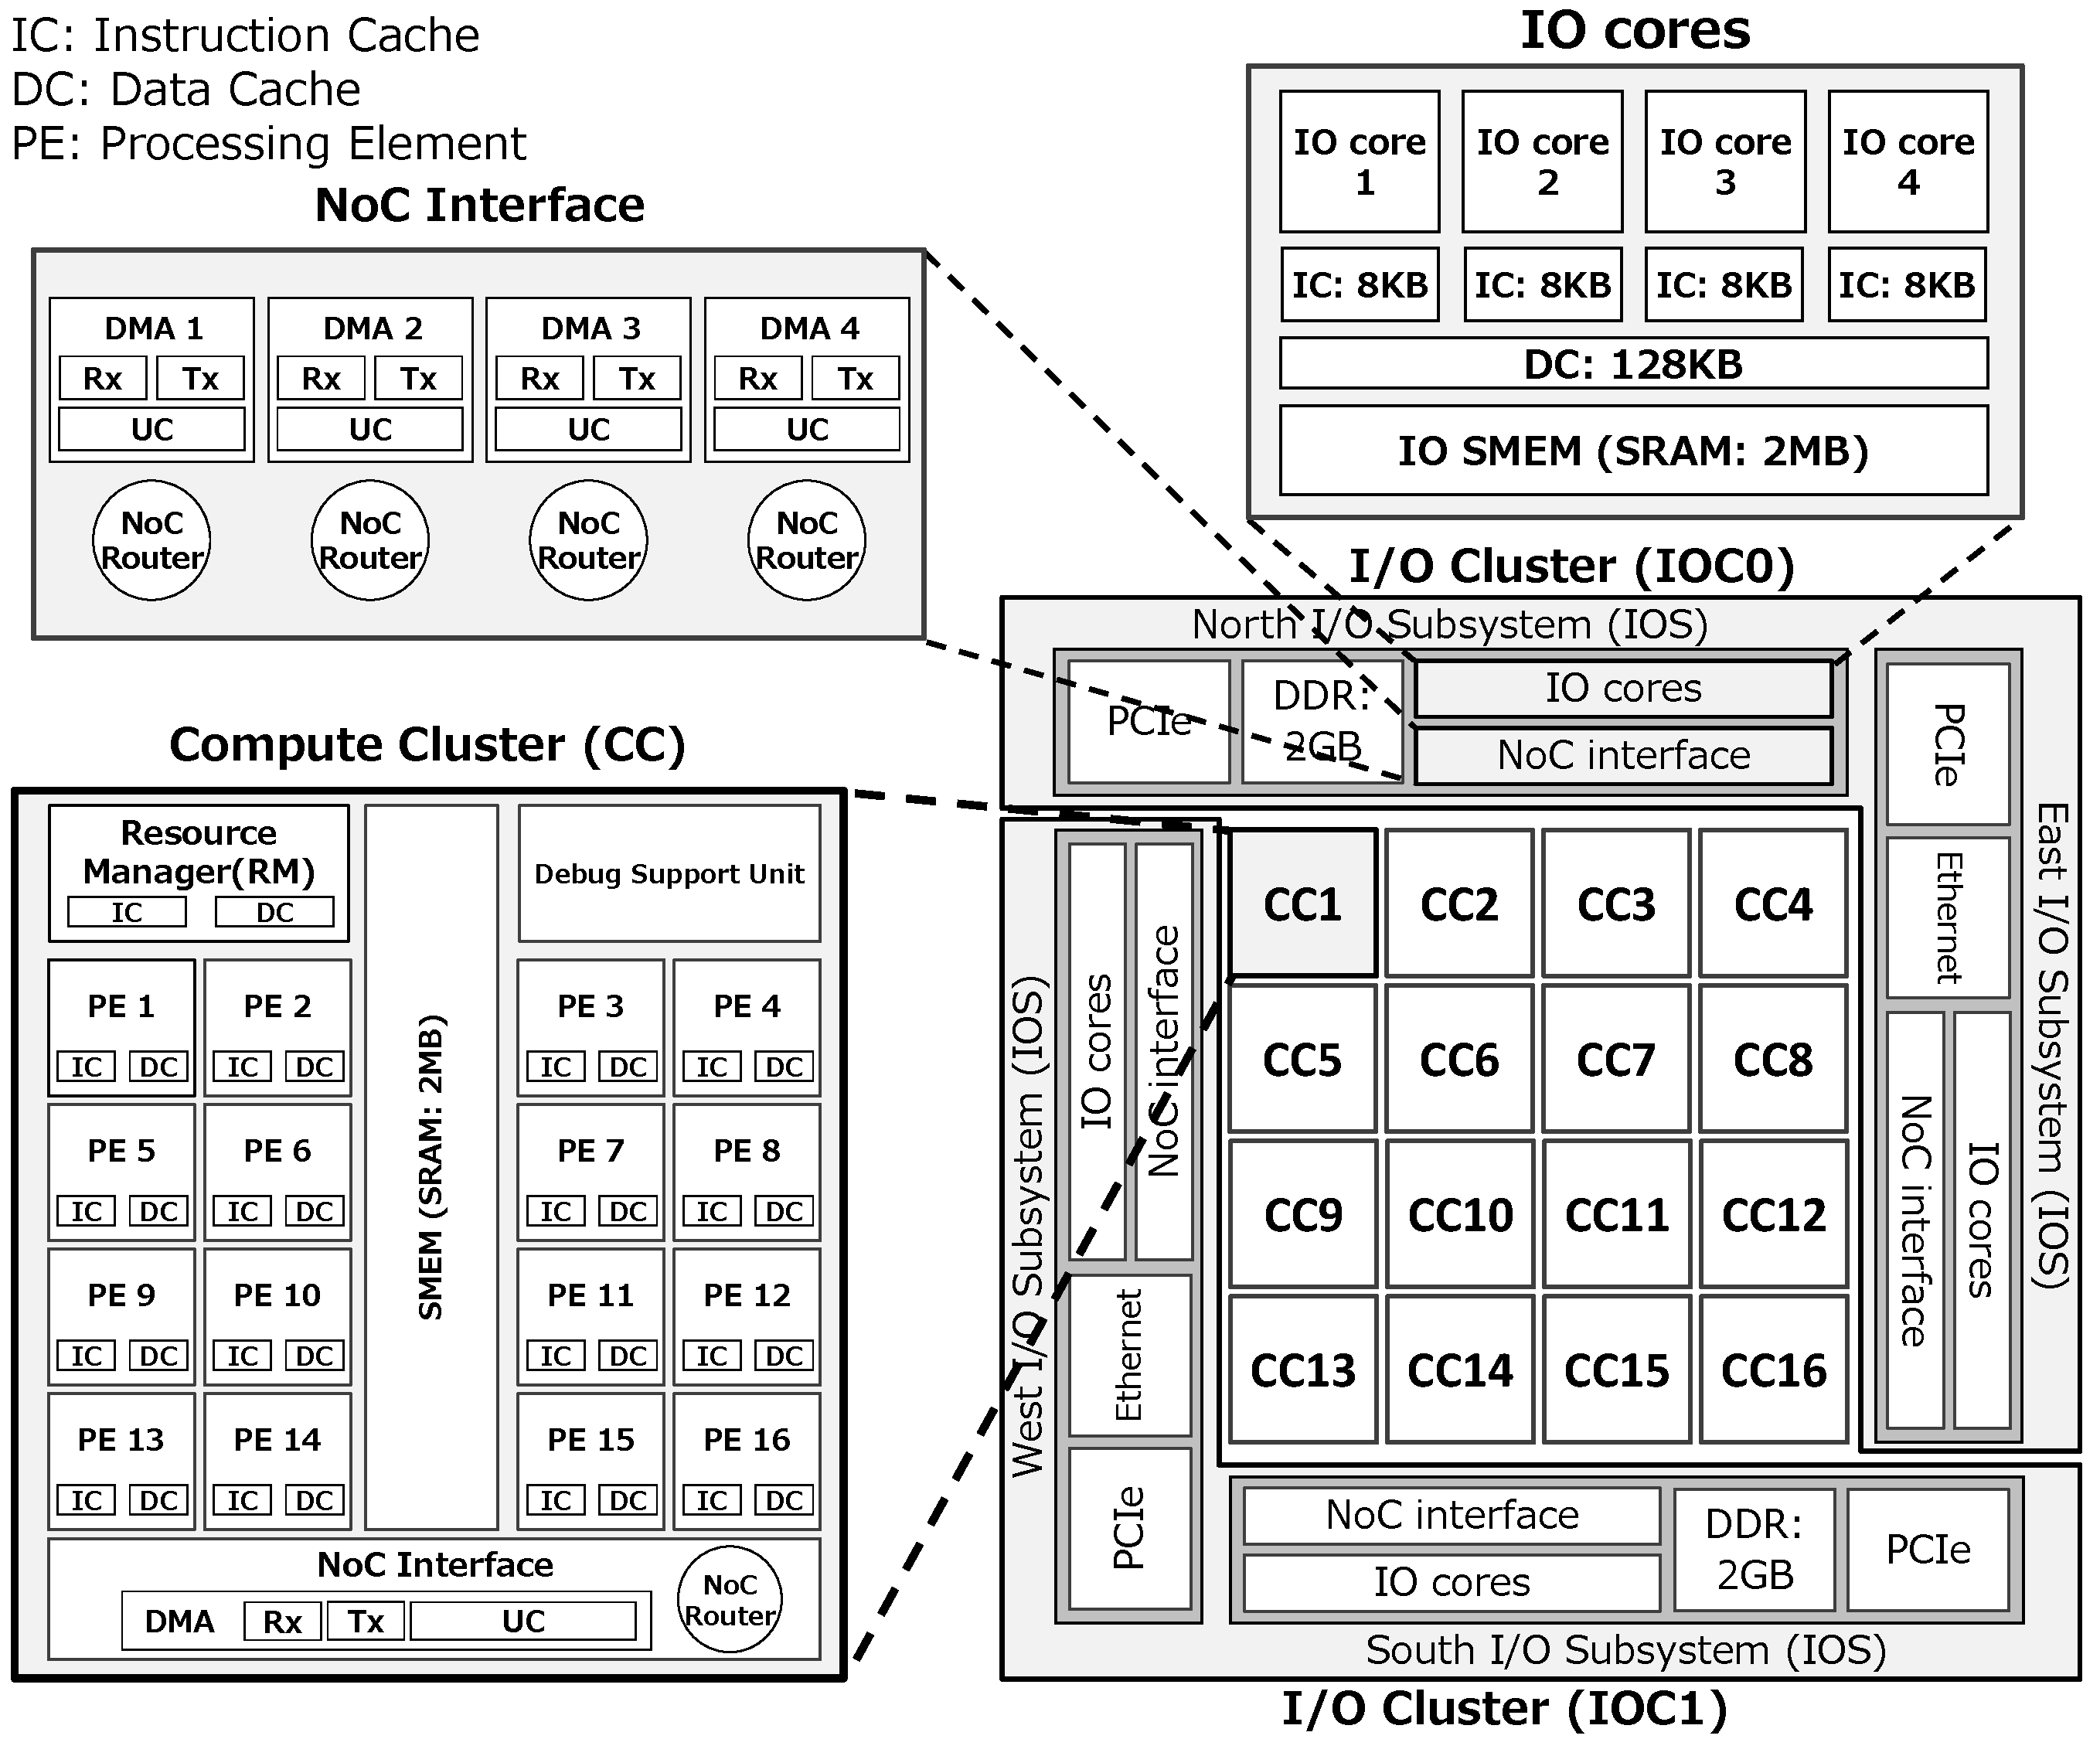
\includegraphics[width=1.0\linewidth]{../figure/mppa_architecture.pdf}
  \caption{\label{fig:mppa_architecture}
    Kalray MPPA-256 Bostanのアーキテクチャの概要}
\end{figure}

\setlength{\headheight}{0pt}

\subsubsection{I/Oサブシステム(IOS)}
\label{sec:ios}
MPPA-256には,北,南,東,西の4つのI/Oサブシステム(IOS)がある.
北と南のIOSは,DDRインタフェースと8レーンのPCIeコントローラに接続されている.
東と西のIOSは,10GB/sイーサネットコントローラに接続されている.
各IOSは4つのI/OコアとNoCインタフェースで構成されており,図\ref{fig:mppa_architecture}のように2つのIOSによって1つのI/Oクラスタ(IOC)が構成される.

\textbf{I/Oコア}:I/Oコアは,図\ref{fig:mppa_architecture}に示すように,合計容量が2MBの共有メモリ(IO SMEM)に接続される.
各I/Oコアは32($ 8 \times 4 $)KBの独自の命令キャッシュを持ち,128KBのデータキャッシュ及び外部のDDRメモリへのアクセスを4つのI/Oコアで共有する.
% 128KBのデータキャッシュを共有することにより,I/Oコア間のコヒーレンシが可能になります.
さらに,I/Oコアは,PCIe,Ethernet,及びその他のI/Oデバイスコントローラ等を管理している.
% これらは,DMAを使用したNoCインタフェースを含むローカルペリフェラルを操作します.

\textbf{NoCインタフェース}:NoCインタフェースは,図\ref{fig:mppa_architecture}のように4つのDMAエンジン(DMA1-4)と4つのNoCルータを持つ.
DMAエンジンは,NoCルータを介したデータ通信を管理しており,受信(Rx)インタフェース,送信(Tx)インタフェース,及びマイクロコア(UC)の3つのNoCインタフェースを備えている.
UCは,マルチスレッドエンジンで,Txインタフェースでデータを送信するスレッドを設定するようにプログラムできる.
設定されたパターンを使用してメモリからデータを抽出し,NoCでデータの送信を開始し,動作後は他のプロセッシングエンジン(PE)及びI/Oコアを利用することなく自律的に実行することが可能である.

\subsubsection{コンピュートクラスタ(CC)}
\label{sec:cc}
MPPA-256では,16個のコアを持つコンピュートクラスタ(CC)が16個存在し,合計256のコアによって主要な処理が行われる.
NoC上の16個の内部ノードがCCに対応しており,図\ref{fig:mppa_architecture}は各CCのアーキテクチャを示している.

\textbf{プロセッシングエンジンとリソースマネージャ}:
CCでは,16個のプロセッシングエンジン(PE)と1個のリソースマネージャ(RM)が2 MBのクラスタローカルメモリ(SMEM)を共有する.
PEは主に,並列処理のためにユーザーによって使用される.
% 開発者はPE上にコンピューティングスレッドを生成します.
CC内のPEとRMは,Kalray独自の32ビットVLIWのKalray-1コア(600MHzまたは800MHz)となっている.
% 各コアには,独自の命令キャッシュとデータキャッシュが装備されています.

\textbf{デバッグサポートユニットとNoCインタフェース}:
SMEMのバスマスタは,PEとRMの他に,デバッグサポートユニットとNoCインタフェース内のDMAエンジンとなる.
DMAエンジンとNoCルータは,NoCインタフェース内に配置されており,CCのDMAエンジンにも,Rx,Tx,及びUCの3つのインタフェースが存在している.

\subsubsection{ネットワークオンチップ(NoC)}
\label{sec:noc}
16個のCCと4つのIOSは,図\ref{fig:noc_map}のようにネットワークによって接続されている.
プロセッサ上にバスネットワークとしてNoCが構築されており,各ノードにはルータが存在する.

\begin{figure}[t]
  \centering
  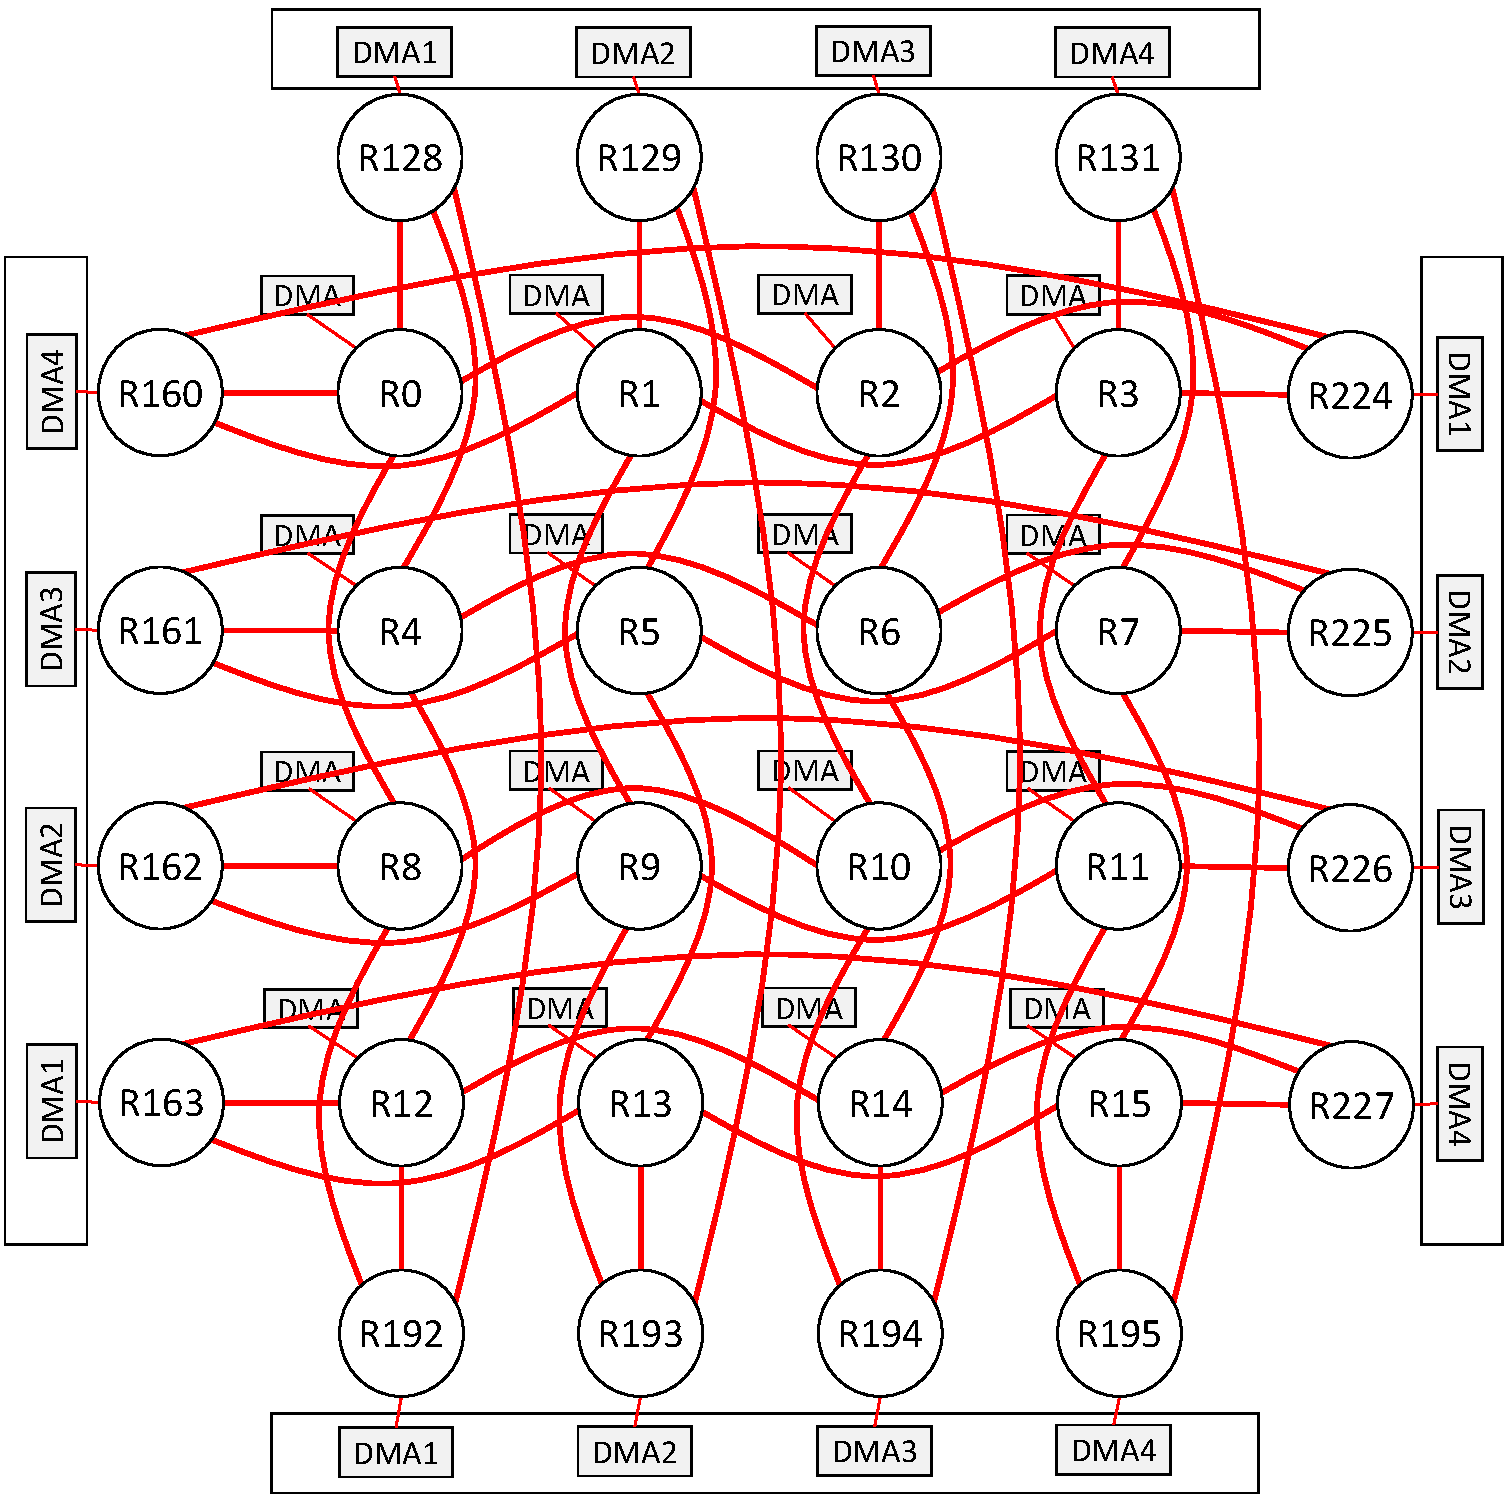
\includegraphics[width=0.65\linewidth]{../figure/noc_map.pdf}
  \caption{\label{fig:noc_map}
    NoC(Network-on-Chip)マップ}
\end{figure}

\textbf{バスネットワーク}:
バスネットワークはノード(CCとIOS)をトーラス状に接続している\cite{dally2001route}.
トーラス状ネットワークのメリットはメッシュ状\cite{vangal200780} \cite{taylor2002raw}の場合と比べて平均ホップ数が少なくなることにある.
実際には,ネットワークは双方向リンク(図\ref{fig:noc_map}に赤線で示される)を持つ2つの並列バスで構成されている.
大きな容量のデータ転送に最適化されたData-NoC(D-NoC)と低レイテンシで小さなメッセージ用に最適化されたControl-NoC(C-NoC)である.
NoC上のデータは,フリットと呼ばれる単位に分割される方式で転送され,ルータ間を循環するデータは可変長フリットによってパッケージ化されている.

\textbf{NoCルータ}:
CCごとの1つノードとIOSごとの4つのノードには,D-NoCルータとC-NoCルータがある.
さらに,CC/IOS上のNoCインタフェースのDMAエンジンは,Rxインタフェース,Txインタフェース,及びUCを備えたD-NoCルータを介して送受信を行う.
図\ref{fig:mppa_architecture}に示されているNoCルータは,図\ref{fig:noc_map}のノードと対応する.
% 簡単にするために,D-NoC / C-NoCルータはNoCルータで示されています.
D-NoCとC-NoCの両方で,各ネットワークノード(CCまたはIOS)には次の5つの方向へのリンクを持っている.
東西南北の4つの隣接リンク及び,及びNoCルータに接続されたローカルアドレススペースへのリンクの計5つである.
NoCルータは,各方向でフリットをFIFOキューイングし,リンク幅は各方向4バイト幅であり,コアが600MHzまたは800MHzのCPUクロックレートで動作するため,各ノードは合計2.4GB/秒または3.2GB/秒で送受信することとなる.

\vspace{-2mm}
\subsection{ソフトウェアモデル}
\label{sec:software_model}

\begin{figure}[t]
  \centering
  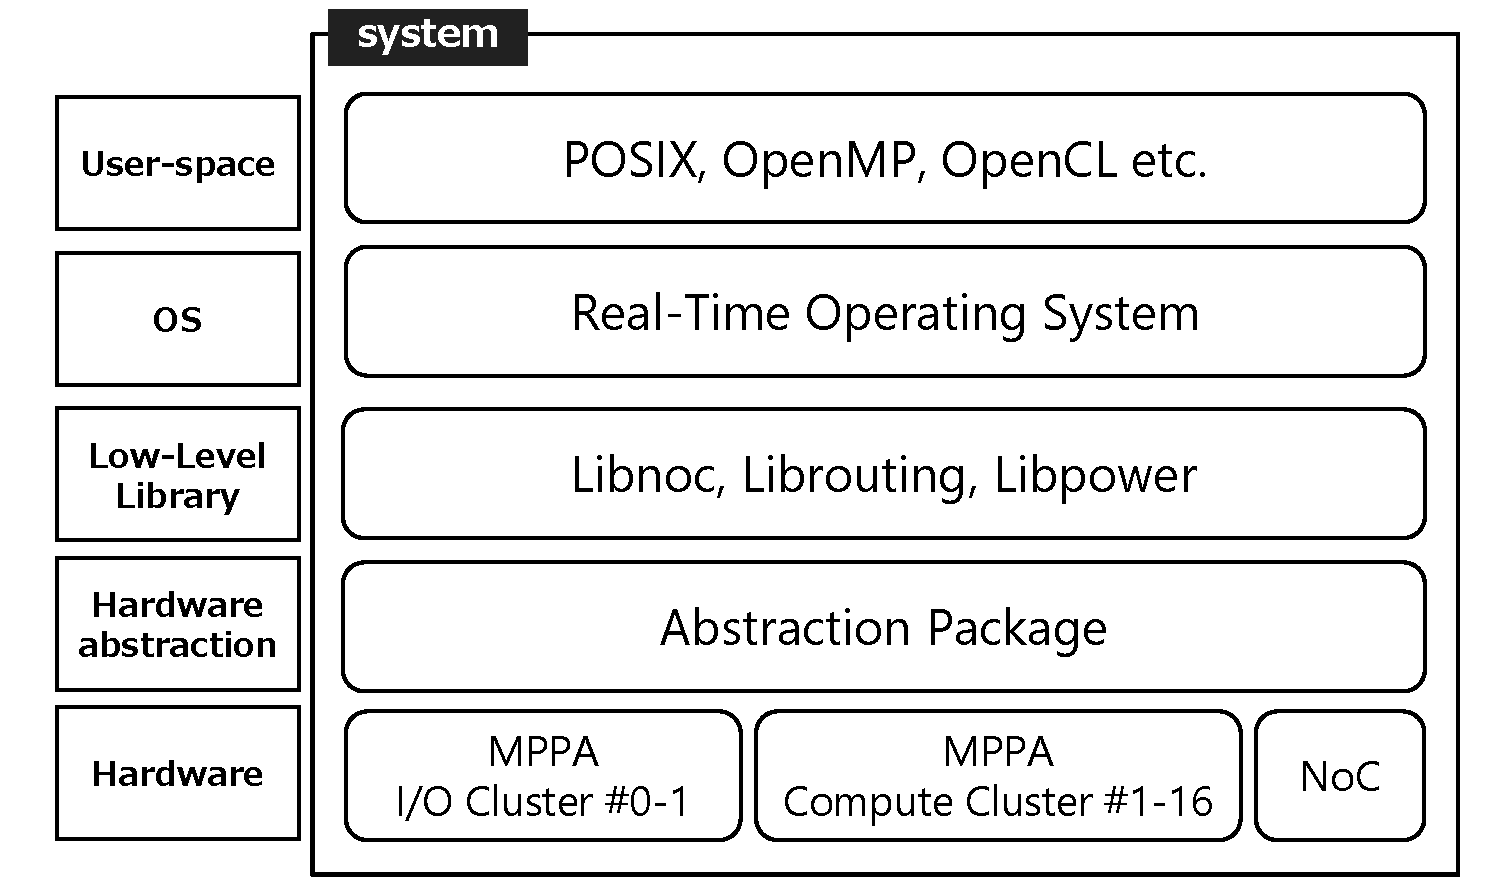
\includegraphics[width=0.8\linewidth]{../figure/softwarestack.pdf}
  \caption{\label{fig:software_stack}
    Kalray MPPA-256のシステム構成}
\end{figure}

図\ref{fig:software_stack}は,本研究で扱うKalray MPPA-256に使用されているソフトウェアスタックを示している.
Linux,リアルタイムOS(Real-Time OS:RTOS),POSIX API,OpenCL,及びOpenMP等のいくつかのプログラミングモデルまたはランタイムをマッピングすることが可能である.

ハードウェア抽象化レイヤでは,抽象化パッケージがCC,IOS,及びNoCのハードウェアを抽象化する.
抽象化は,ハードウェアリソースを分割し,ユーザー空間のOSライブラリからのリソースへのアクセスを制御している.
% これは,パーティション間通信を設定し,仮想マシン抽象化レイヤーとして制御します.
ハードウェア抽象化は主にRMコアで実行される.
% すべてのサービスは,ユーザ空間ライブラリによって提供されなければならないオペレーティングシステム(例えば,仮想メモリ及びスケジュール)によって一般的に提供される.
% カーネルが最小限に抑えられているため,リソースの浪費やニーズの不一致が回避されます.

低レベルのライブラリ層では,Kalrayの提供するシステムがNoCを処理するためのライブラリを提供している.
さらに,NoCのルーティングやQoS等の機能は,プログラマによって設定可能となっている.
Libnocは,メモリマップレジスタへの直接アクセスを可能にし,最低限のオーバヘッドで設計されてる.
Libroutingは,MPPAの任意のクラスタ間でのデータ通信をルーティングするための最小限の機能を提供する.
このライブラリではトーラスネットワーク上のルーティングは独自のポリシーで静的に実行されており,必ずしも最小のホップ数を保証するものではない.
Libpowerを使用すると,リモートクラスタの起動や実行終了を待機することができる.

さらに,OS層の抽象化パッケージは様々なOSをサポートしている.
ここでは,その中からRTOSであるeMCOSを紹介する.
eMCOSは日本のRTOSのサプライヤであるeSOLによって開発されたリアルタイム組込みOSであり,eMCOSは世界で初めて市販された組込みシステム向けメニーコアRTOSである.
CCとIOSの両方で動作し,最小限のプログラミングインタフェースとライブラリを提供する.
eMCOSは分散マイクロカーネルアーキテクチャを実装しており,これにより,アプリケーションは優先順位ベースのメッセージパッシング,ローカルスレッドスケジューリング,スレッド管理をIOS及びCCで操作することが可能になっている.

% \textbf{RTEMS}: RTEMS(マルチプロセッサシステム用リアルタイムエグゼクティブ)は,組込みプラットフォーム用に用意されたフル機能のRTOSです.
% これはいくつかのAPIと標準をサポートしており,特にPOSIX APIをサポートしています.
% RTEMSは,CCを除くIOC上で動作します.

% \textbf{NodeOS}:CCでは,MPOSAクラスタオペレーティングシステムはNodeOSというランタイムを使用します.
% OSはマルチコアOSが標準のPOSIX APIに可能な限り対応できるようにする必要性に対処しています.
% NodeOSは,POSIX APIを使用してCC上のPEで実行することにより,ユーザーコードを有効にします.

% \textbf{eMCOS}:CCとIOSの両方で,eMCOSは最小限のプログラミングインタフェースとライブラリを提供します.
% 具体的には,eMCOSはeSOL(日本のRTOSのサプライヤ)によって開発されたリアルタイム組込みオペレーティングシステムであり,eMCOSは組込みシステム向けの世界で初めて市販されている多コアRTOSです.
% OSは分散マイクロカーネルアーキテクチャを実装しています.
% これにより,アプリケーションは優先順位ベースのメッセージパッシング,ローカルスレッドスケジューリング,及びスレッド管理をIOS及びCCで操作できます.

\begin{figure}[t]
  \centering
  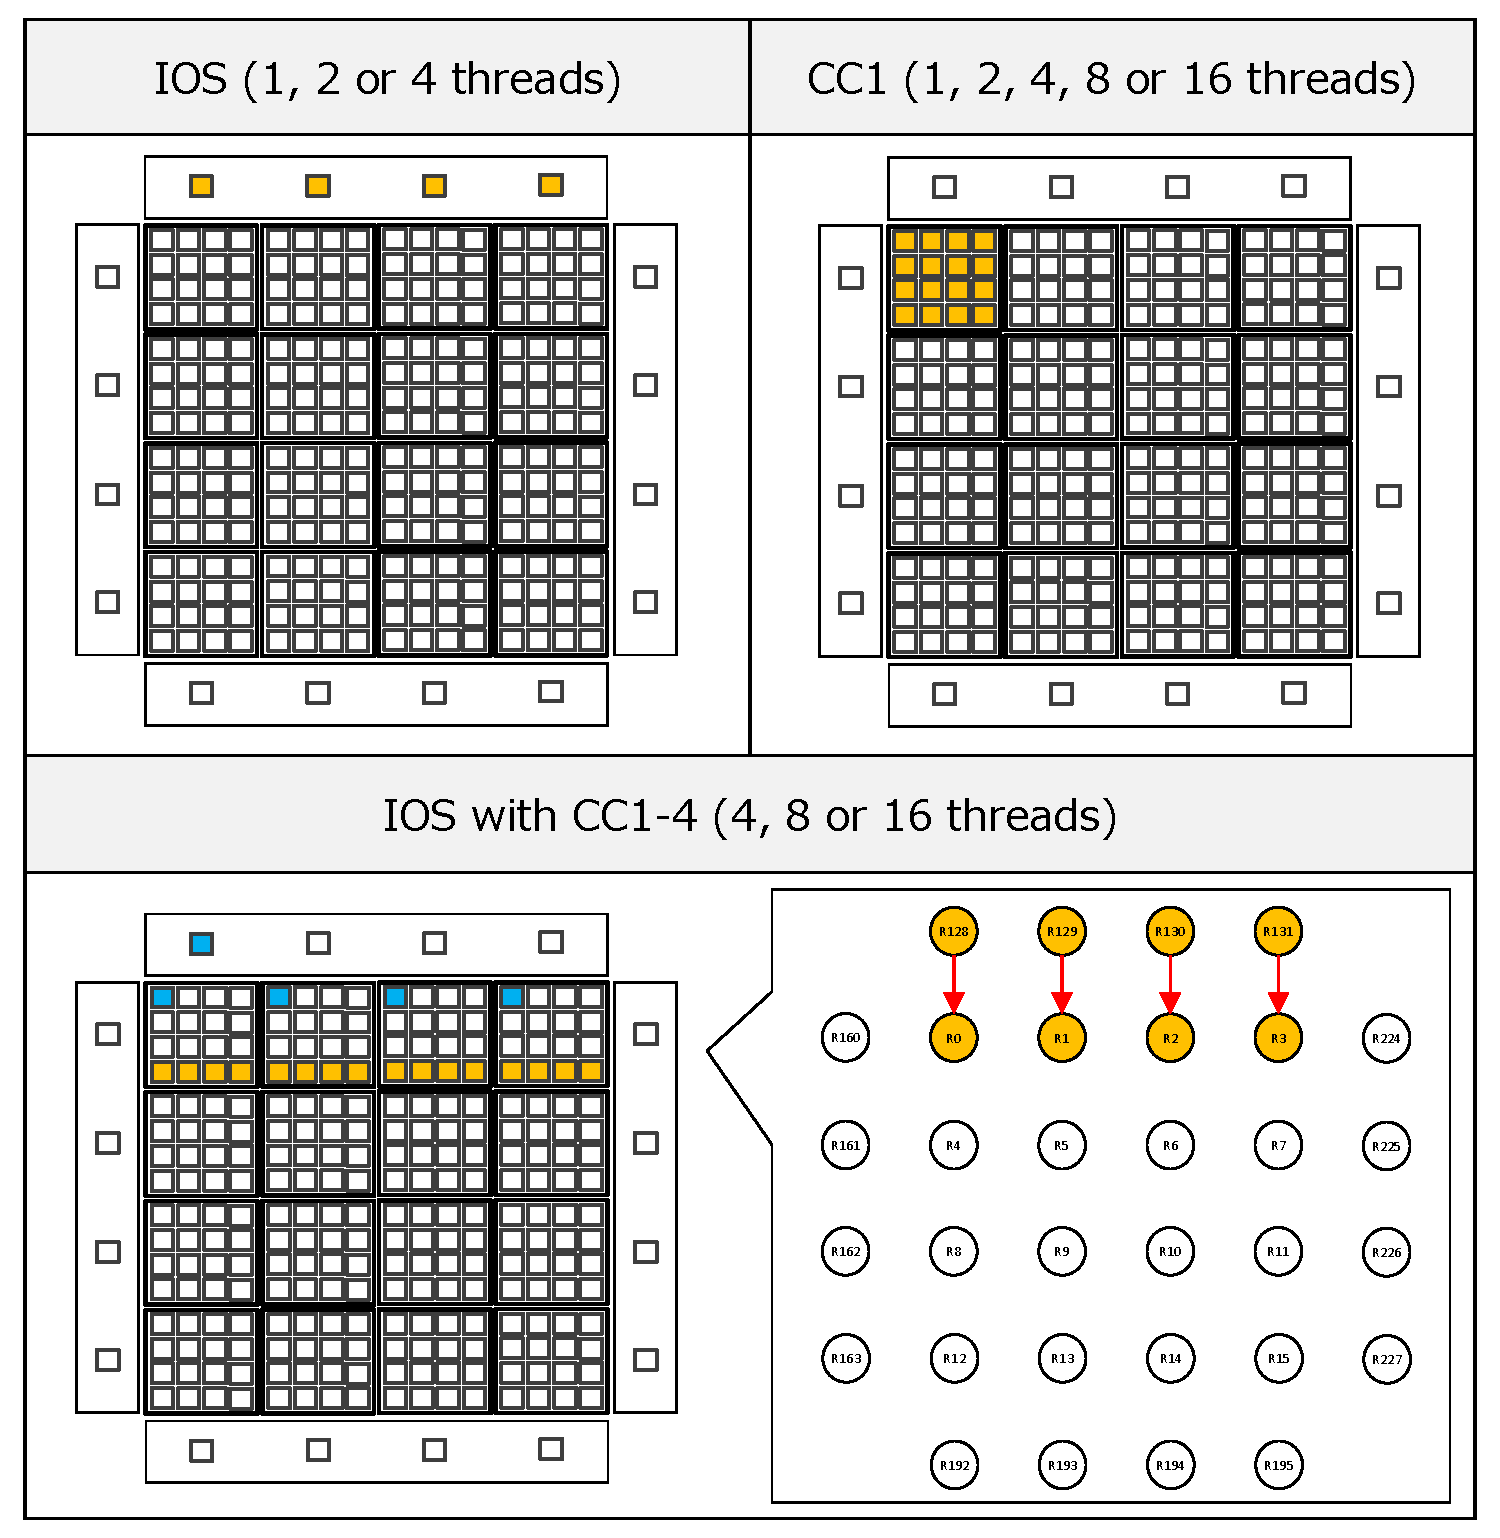
\includegraphics[width=0.8\linewidth]{../figure/matrix_calculation.pdf}
  \caption{\label{fig:mat_calc}
    行列計算の評価構成}
\end{figure}

\section{評価と考察}
\label{sec:evaluations}
本章ではまず,MPPA-256の並列化可能性とメモリアクセス特性を示すための行列計算の評価を行う.
その後,NUMAのメニーコアの実用性を検証するため,実用的な自動運転アプリケーションの並列化を行い,最後に全体の考察を行う.
以下のすべての評価実験は,eMCOSを使用した実際のハードウェアボード上で行われるものとする.

% \subsection{D-NoC Data Transfer}
% \label{sec:dnoc_eval}
% \subsubsection{Situations and Assumptions}
% \label{sec:situations_and_assumptions}
% \subsubsection{Data Transfer Methods}
% \label{sec:data_transfer_methods}
% \subsubsection{Influences of Routing and Memory Type}
% \label{sec:routing_and_memory}

\vspace{-2mm}
\subsection{行列計算}
\label{sec:martix_eval}

\subsubsection{評価構成と仮定}
\label{sec:situations_and_assumptions}
本評価では,MPPA-256の行列計算時間を計測する.
行列計算はIOSとCCで行われ,図\ref{fig:mat_calc}に示すように,3つの計算ケースが想定する.
第一のケースでは,IOS内で4つのコアを用いて計算される.
ここでは,メモリアクセス特性を分析するために,IO DDR及びSMEMに行列バッファを割り当てる.
第二のケースでは,1つのCCを用いて,1~16コアで計算を行う.

そして,第三のケースでは,IOSと4つのCCを使用してオフロードコンピューティングを行う.
ここでは,IOSとCCのいくつかのコアは,行列計算とは別に,並列化された処理の管理を担っている.
このケースでは,4つのCCを用いるため,SMEMによる2MBの制約がなく,分散メモリを用いて2MBを超えるデータを処理することが可能である.
また,IOS及びCCのコアは,キャッシュのコヒーレンシトラブルを回避するために,キャッシュを無効にした状態で行列バッファにアクセスする必要がある.
NoCでのデータ通信については,図\ref{fig:mat_calc}に示すように行列バッファを4つのDMAで分担して並列送信を行った.

各ケースでの行列計算時間は,並列化の度合いと割り当てられたメモリの種類,キャッシュのON/OFFの3つの観点で分類される.
以下の評価では,OS等のシステムアプリケーションのメモリ領域も考慮し,利用可能な合計バッファサイズは1MBとした.
したがって314KBの行列を3つ準備し,行列Aと行列Bが乗算され,結果が行列Cに格納されるものとする.
また,第三のケースに関しては,メモリの制約が一部解除されるため,640KBの行列による計算も行った.

\subsubsection{キャッシュとメモリの種類の影響}
\label{sec:cache_and_memory}

\begin{figure*}[t]
  \tabcolsep = 0.5mm              % side-margin in column
  \begin{tabular}{cc}
    \begin{minipage}[t]{0.49\textwidth}
    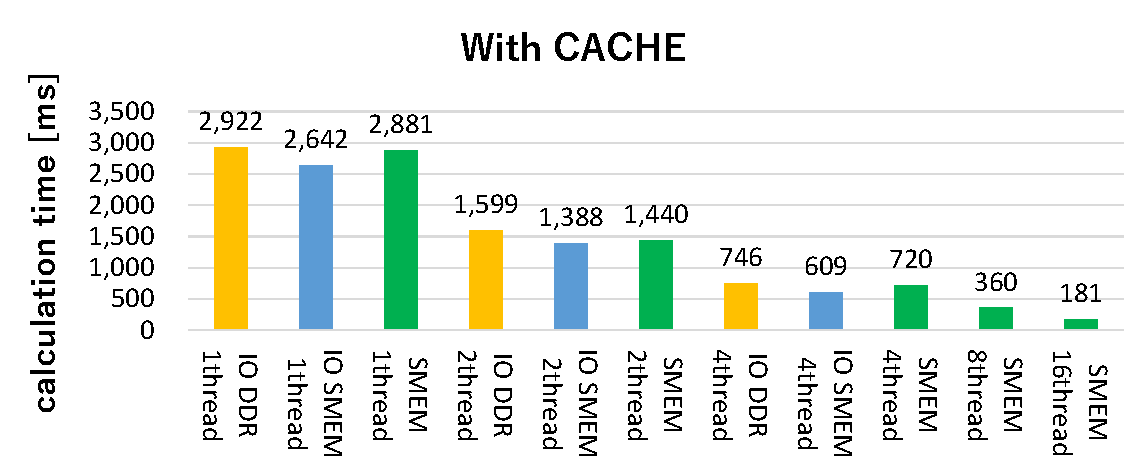
\includegraphics[width=1.0\linewidth]{../figure/BarGraph_matrix_with_cache.pdf}
      \caption{行列計算:IOSとCC(キャッシュ有効)}
      \label{fig:mat_calc_cache}
    \end{minipage}   
    &
    % \setcounter{figure}{11}
    \begin{minipage}[t]{0.49\textwidth}
      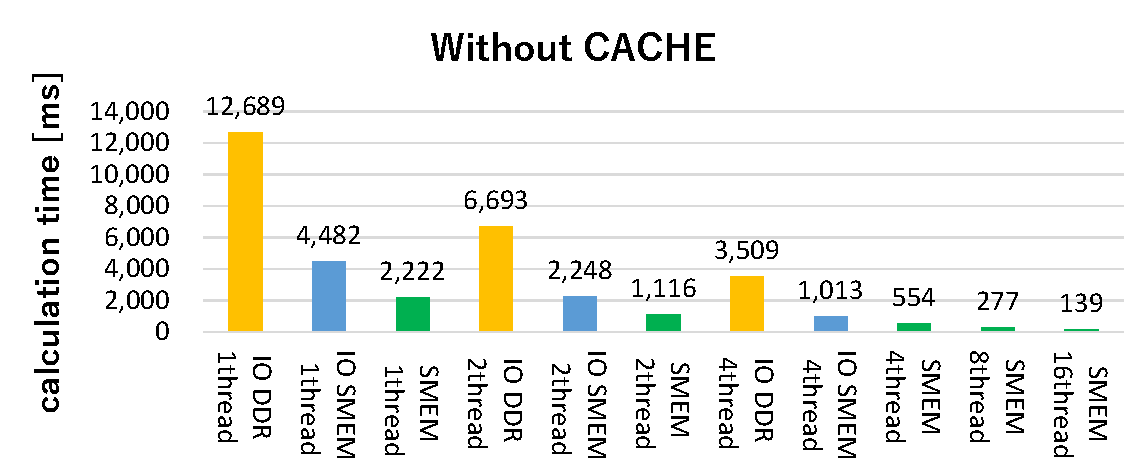
\includegraphics[width=1.0\linewidth]{../figure/BarGraph_matrix_without_cache.pdf}
      \caption{行列計算:IOSとCC(キャッシュ無効)}
      \label{fig:mat_calc_uncache}
    \end{minipage}
    % \vspace{-3mm}
  \end{tabular}
  \vspace{-2mm}
\end{figure*}

IOSとCCでキャッシュを有効した場合の行列計算の結果を図\ref{fig:mat_calc_cache}に示す.
IO DDR,IO SMEM,及びCC SMEMは,キャッシュによってほとんど違いがないことが分かる.
これは,IOSの128 KBのデータキャッシュが機能し,DDRアクセスの遅延を補っていると考えられる.
さらに,計算時間はスレッドの数とほぼ線形関係にあることが観察され,並列化に関する理想的な動作に相当する.

次に,IOSとCCのキャッシュを無効にした場合の行列計算の結果を図\ref{fig:mat_calc_uncache}に示す.
キャッシュを無効にしたことで,DDRでの計算時間が約4倍に増加し,SMEMと比較して大きな差が生じている.
他の特筆すべき結果は,CC SMEMの計算速度がIO SMEMの計算速度を超えていることである.
この特性は,キャッシュ有効時の結果(図\ref{fig:mat_calc_cache})では隠れている特性である.
計算を行っているコア自体はIOSとCCでは物理的には同じなので,SMEMの特性や物理的配置が大きな影響を及ぼしていると考えられる.
CC SMEMとIO SMEMに無視できない大きな差が存在することは,興味深い結果である.
さらに,計算時間はスレッド数と線形関係にあることも観察され,CC SMEMにおけるキャッシュ無効時の計算速度は,キャッシュ有効時の計算速度を上回っている.
キャッシュ有効時にアクセス速度が遅くなることは直感に反するものであり,可能性としてはキャッシュラインの問題が考えられる.
CCのPE内の小型データキャッシュ(8KB)が十分に機能せず,アプリケーションが頻繁にキャッシュのミスヒットを起こした場合,メモリアクセスはキャッシュされていないデータアクセスの時間とキャッシュラインを補充するためのコストを同時に支払うことになる.
その結果,キャッシュ無効時のメモリアクセス速度がキャッシュ有効時のメモリアクセス速度を超えていると考えられる.

\subsubsection{4つのCCによる並列化}
\label{sec:four_CCs}

\begin{figure*}[t]
  \tabcolsep = 0.5mm              % side-margin in column
  \begin{tabular}{cc}
    \begin{minipage}[t]{0.49\textwidth}
      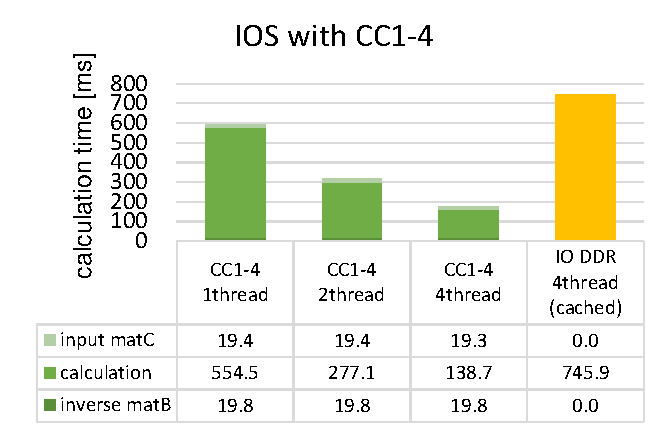
\includegraphics[width=0.9\linewidth]{../figure/BarGraph_matrix_with_CCs_314.pdf}
      \vspace{-2mm}
      \caption{行列計算:IOS + 4 CCs(314KB 行列 \(\times\) 3)}
      \label{fig:mat_calc_offload_314}
    \end{minipage}   
    &
    % \setcounter{figure}{11}
    \begin{minipage}[t]{0.49\textwidth}
      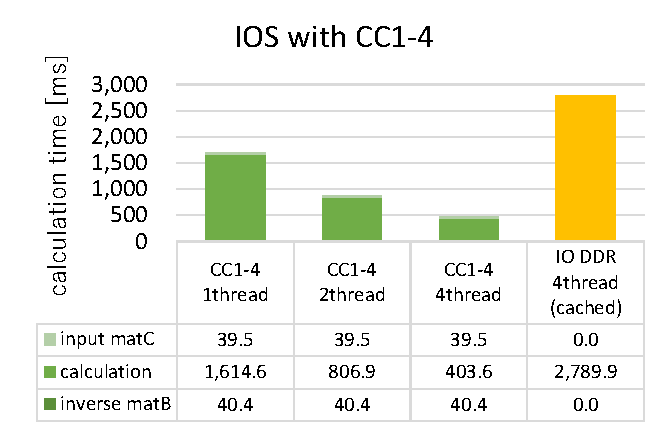
\includegraphics[width=0.9\linewidth]{../figure/BarGraph_matrix_with_CCs_640.pdf}
      \vspace{-2mm}
      \caption{行列計算:IOS + 4 CCs(640KB 行列 \(\times\) 3)}
      \label{fig:mat_calc_offload_640}
    \end{minipage}
    % \vspace{-3mm}
  \end{tabular}
  \vspace{-2mm}
\end{figure*}

最後に,IOSとCCでのオフロードコンピューティングによる行列計算の結果を図\ref{fig:mat_calc_offload_314}に示す.
この場合,行列バッファの合計容量が1MBを超えると仮定し,計算速度の結果はIO DDR(キャッシュ有効時)と比較することになる.
並列化に伴い,IOSでは,行列バッファのCCへ転送処理や送信バッファに詰めるための行列の転置計算(inverse matB),各CCでの計算結果を受け取った後に結果を行列バッファに集約するための処理(input matC)等が余分に必要になる.
これらは,図\ref{fig:mat_calc_offload_314}と図\ref{fig:mat_calc_offload_640}に示されるように,一定のオーバヘッドを生んでいる.
しかし,オーバヘッドを考慮しても,オフロードによる計算速度は,IO DDR(キャッシュ有効時)の速度を上回っている.
この結果は,いくつかの重要な事実を示している.
第一に,D-NoCデータ転送は計算時間に比べてオーバヘッドをほとんど発生させていない.
第二に,DDRへのDMAメモリアクセスの速度は,I/Oコアのメモリアクセスの速度を超えている.
オフロードの場合,DMAはDDRの行列バッファにアクセスし,IO DDRから各CC SMEMにデータを転送する.
その後,CC内のPEは,キ ャッシュを無効にした状態で行列バッファにアクセスすることになる.
MPPA-256の場合,NoCのデータ通信とDMAによるメモリアクセスのオーバヘッドが少なく,並列化されたNoCデータ通信と複数のCCによる分散メモリが実用的であるといえる.
% そして,図\ref{fig:mat_calc_offload_640}に示すように,行列サイズが大きい場合,オフロードの影響が大きくなります.
% これらのオフロード評価では,各CCが同時に計算結果をIOSに送信します.
計算結果が格納されている行列CをDDRに配置した場合,DDRのメモリアクセス遅延によりNoCルータのFIFOがオーバフローし,エラーが発生することが観測された.
図\ref{fig:mat_calc_offload_314}, 図\ref{fig:mat_calc_offload_640}の評価結果は,行列CがDDRで割り当てられている場合の結果であるが,このエラーは伝送プロトコルによって防止されるべきであり,NoC上でフリットのフロー制御はMPPA-256の今後の課題である.
現在,このエラーを確実に回避するには,行列CをIO SMEMに割り当てる必要がある.

\subsection{実アプリケーション}
\label{sec:practical_application}
本節では,自動運転システムの一部のアルゴリズムを採用し,組込み向けメニーコアプラットフォームの実用性を検証する.
本研究では,市街地自動運転のためのオープンソースソフトウェアであるAutoware\cite{kato2015open}のC++で記述された車両の自己位置推定アルゴリズムの並列化を行った.
アルゴリズムは,主にPoint Cloud Library\cite{pcl}に実装されているいる正規分布変換マッチングアルゴリズム\cite{magnusson2009three}を採用している.

自己位置推定アルゴリズムのボトルネック部分は主に\emph{computeTransform}関数であり,レーザセンサからのスキャンクエリごとに最大8個の近傍点を地図データから探索し,ニュートン法により位置推定結果が収束するまで処理を繰り返す関数になっている.
この評価実験では,\emph{computeTransform}の一部を16個のCCで並列化し,残りの部分をIOS上の4つのコアで並列化した.
探索対象となる地図データが1MBを超えるため,\emph{computeTransform}関数全体をCCで並列化するには,最近傍点探索のアルゴリズム自体を大きく再設計する必要がある.
このアルゴリズムの再設計はNUMA採用によるデメリットといえ,今後の課題のひとつである.

並列化された自己位置推定アルゴリズムの評価を,図\ref{fig:ndt_matching}に示す.
推定結果収束までの平均実行時間を計測し,並列化によって\emph{computeTransform}関数が高速化されているを示している.
現状では多くの自動運転システムにおいて,レーザセンサからスキャンクエリは10Hzとなることが多く,今回の並列化によりデッドラインとなる100ミリ秒以下を達成したことになる.
この並列化されたアルゴリズムは,シミュレーションと実車実験の両方で動作実験が行われ,テストコース内で正常に動作することが確認されている.

\begin{figure}[t]
  \centering
  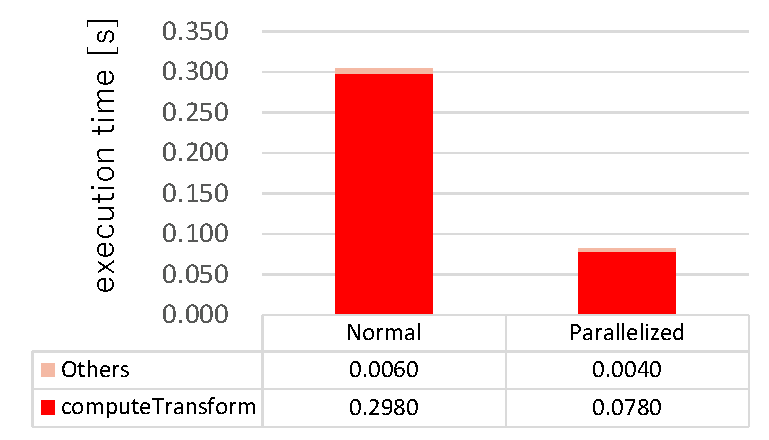
\includegraphics[width=0.9\linewidth]{../figure/BarGraph_ndt_matching.pdf}
  \vspace{-2mm}
  \caption{\label{fig:ndt_matching}
  MPPA-256による自動運転システムの自己位置推定処理の並列化}
  \vspace{-2mm}
\end{figure}


\subsection{考察}
\label{sec:lessons}
本章では,NoCベースの組込みメニーコアのデータ転送と並列コンピューティングの特性を明らかにしてきた.
これらの実験結果から,MPPA-256を始めとするNoCベースのメニーコアプラットフォーム使用者及び開発者のためのガイドラインを得ることができる.

% D-NoCデータ転送の評価から,NoCルーティングとDMAの2つのレッスンが得られます.
% 第1に,クラスタ間のデータ転送レイテンシは,図8に示すように,ユーザのためのルーティングの影響をほとんど受けない.図8に示すように,\ref{fig:DDR_uc},\ref{fig:IO_SMEM_tx},及び\ref{fig:IO_SMEM_uc} .
% ルータ及びRMにおける送受信のソフトウェアトランザクションは,待ち時間の主な要因です.
% 第2に,IOSでは,UCのレイテンシは,転送されたバッファが図\ref{fig:tx_uc_log}の評価から割り当てられたメモリ位置,DDRまたはSMEMの影響をあまり受けない.
% UCを使用すると,特に大きなデータの場合,DDRからCC SMEMにデータを転送するのが一般的な状況であるため,UCのメリットはユーザーにとって有益です.

行列計算のマイクロベンチマークからは,SMEMの特徴,キャッシュの影響,D-NoCのデータフロー制御の3つのメモリアクセスに関する考察を得ることができる.
まず,CC SMEMのメモリアクセス速度は,図\ref{fig:mat_calc_uncache}のようにIO SMEMのメモリアクセス速度を超えていることである.
ここには無視できない差異が存在し,CCで積極的に処理をするための大きな根拠となる.
次に,図\ref{fig:mat_calc_uncache}のCC SMEMでのキャッシュ無効時の計算速度が,図\ref{fig:mat_calc_cache}のキャッシュ有効時のものを上回っていることを定量的に示したことが挙げられる.
キャッシュのミスヒットが頻繁に発生した場合,オーバヘッドが存在することは一般的に知られているが,キャッシュラインの影響によって無視できない大きな差異が発生することは特筆すべき項目といえる.
最後に,データが複数のCCからIO DDRに並列転送される場合,DDRへのメモリアクセス遅延のためにIOS内のNoCルータのFIFOがオーバフローする問題である.
これは,今後,伝送プロトコルとフロー制御によって防止する必要がある.

\ref{sec:practical_application}章の実アプリケーションによる評価では,自動運転システムの自己位置推定アルゴリズムを並列化し,実用化可能性を示した.
CC SMEMをスクラッチパッドメモリとして使用したNoCによるIOSからCCへのデータ転送やIOS/CCでの並列コンピューティングは実際の複雑なアプリケーションにも応用可能であるといえる.

\section{関連研究}
\label{sec:related_work}
本章では,MPPA-256と他のマルチ/メニーコアプラットフォームを比較し,メニーコアに関連する既存研究の紹介を行う.
初めに,本研究で利用したKalray MPPA-256を他のマルチ/メニーコアコンポーネントと比較してMPPA-256の特徴を整理し,続いて本研究と既存研究との比較を行う.

% テーブル\ref{tb:comparison_platforms}は,多くのコアのプラットフォームと他のプラットフォームの機能をまとめたものです.
% 例えば,GPUはコンピューティング性能を向上させる強力な装置であり,特定の分野(例えば画像処理,学習等)において大きな可能性を秘めている.
% しかし,主に特定の目的に使用されており,その予測可能性はリアルタイムシステムには適していません.
% 多くの種類のアプリケーションにGPUを使用し,GPUアーキテクチャのためにその信頼性を保証することは困難です.
% CPUに基づく多くのコアプロセッサは,ソフトウェアプログラマビリティ及びタイミング予測可能性に関してGPUよりも著しく優れています.
% さらに,MPPA-256等の多くのコアプラットフォームでは,妥当な電力消費が必要であることが一般的に知られています(kanter2015kalray).
% 対照的に,GPUはかなりの電力を消費し,かなりの熱を発生する.
% これは組込みシステムにとって重大な問題です.
% FPGAは,CPUと比較しても高性能デバイスです.
% それらは電力消費に関して効率的である.
% FPGAは予測可能性と効率的な処理を保証します.
% しかし,DSPは,多くの種類のアプリケーションやプログラミングに使用することはできません.
% しかし,FPGAはソフトウエア開発者にとっては難しく,ソフトウエアのモデルがCPUのものと大きく異なるので,CPUの代用品ではない.
% 多くのコア・プラットフォームは,プログラミングとスケーラビリティーの容易さを備えているため,シングル/マルチコアCPUを置き換える可能性があります.

% % \renewcommand{\arraystretch}{1.2}
% \begin{table}[t]
%   \caption{\label{tb:comparison_platforms}
%     Comparison of Many-core to CPU, GPU, and FPGA}
%   % \vspace{-3mm}
%   \centering
%   \scriptsize	                    % text size
%   \tabcolsep = 0.4mm              % side-margin in column
%   \begin{tabular}{c|cccccccccc}
%     \hline
%     & \multirow{2}{*}{performance} & \multirow{2}{*}{power/heat} & \multirow{2}{*}{predictability} & \multirow{2}{*}{real-time} & software & \multirow{2}{*}{costs} & multiple\\
%     &&&&& development && instruction \\
%     \hline
%     \hline
%     CPU & & L & \(\checkmark\) & \(\checkmark\) & \(\checkmark\) & \(\checkmark\) & L \\
%     GPU & \(\checkmark\) &  & L &  & L & \(\checkmark\)\\
%     % DSP & L & L & \(\checkmark\) & \(\checkmark\) & L & \(\checkmark\) & \\
%     FPGA & \(\checkmark\) & L & \(\checkmark\) & L &  & L & \\
%     Many-core & \(\checkmark\) & \(\checkmark\) & \(\checkmark\) & \(\checkmark\) & \(\checkmark\) & L & \(\checkmark\) \\
%     \hline
%   \end{tabular}
%   \begin{flushright}
%      \textasteriskcentered In a table, ``L'' means ``limited''.
%   \end{flushright}
%   % \vspace{-5mm}
% \end{table}

現在,多くのマルチ/メニーコアコンポーネントが開発され,様々なベンダーによってリリースされている.
例えば,KalrayのMulti-Purpose Processing Array(MPPA)-256 \cite{de2014time}やTileraのTile-Gx \cite{ramey2011tile} \cite{schooler2010tile},Tile64 \cite{bell2008tile64},IntelのXeon Phi \cite{chrysos2014intel} \cite{chrysos2012intel},Single-chip Cloud Computer(SCC)\cite{baron2010single})等が挙げられる.
本研究では,リアルタイム組込みアプリケーション向けに設計されたKalray MPPA-256に焦点を当てた.
MPPA-256は,エネルギー効率の高い256個の汎用コアを内包しており,NoCベースのクラスタ構造を持っていることが大きな特徴である.

MPPA-256は,コア数の拡張性と電力効率の面で,他のCOTSマルチ/メニーコアコンポーネントよりも優れている(表\ref{tb:comparison_manycore}参照).
他のプラットフォームとコア数を比較すると,MPPA-256は256コアであるのに対し,他のマルチ/メニーコアコンポーネントは多いものでも64コアとなっている.
この優位性は,16のクラスタがそれぞれ独自のローカル共有メモリを持っているNUMAメモリアーキテクチャに起因している.
MPPA-256を除く多くのプラットフォームでは,すべてのコアがグローバルなDDRメモリを共有しており,特定のバスルートに大きな負荷がかかる.
このため,メモリへのアクセス競合が頻繁に発生し,コア数増加の妨げとなっている.
MPPA-256のNUMAメモリアーキテクチャは上記の問題を軽減し,コア数の拡張性を向上させている.

一方で,NUMAメモリアーキテクチャはコア数の拡張は容易だが,利用可能なメモリ容量を制限し,NoCでのDDRからのデータ転送を必要とすることになる.
特に,多くのメモリを必要とするアプリケーションの場合,既存コードの移植が困難になることが多い.
そのため,表\ref{tb:comparison_manycore}に示されているように,他のCOTSプラットフォームに比べてコードの移植性の観点では劣っている.

電力効率の面では,MPPA-256はコアの数が多いにもかかわらず,優れたエネルギー効率を実現する \cite{kanter2015kalray}.
MPPA-256の1ワットあたりの合計クロック数は,現在のマルチ/メニーコアコンポーネントの中で最も高く,消費電力は,600MHzの場合で16W,800MHzで24Wであり,組込み向けの側面が強くなっている.
MPPA-256は自動車や航空機といった組込み向けメニーコアプラットフォームとして広く受け入れられており,これまでも多くの既存研究で利用されてきている \cite{carle2014static} \cite{perret2016mapping} \cite{perret2016predictable}.

% \renewcommand{\arraystretch}{1.2}
\begin{table}[t]
  \caption{\label{tb:comparison_manycore}
    マルチ/メニーコアプラットフォームの比較}
  % \vspace{-3mm}
  \centering
  \scriptsize	                    % text size
  \tabcolsep = 1.5mm              % side-margin in column
  \begin{tabular}{c|cccc}
    \hline
    & コア数の拡張性 & 電力効率  & コードの移植性 & \\
    \hline
    \hline
    Kalray MPPA-256 \cite{de2014time} & \(\bigcirc\) & \(\bigcirc\) & \(\triangle\) & \\
    Tilera Tile series \cite{bell2008tile64} &  & \(\triangle\) & \(\bigcirc\) & \\
    Intel Xeon Phi \cite{chrysos2014intel} \cite{chrysos2012intel} &  &  & \(\bigcirc\) & \\
    Intel SCC \cite{baron2010single} &  &  & \(\bigcirc\) & \\
    \hline
  \end{tabular}
  % \vspace{-5mm}
\end{table}

既存研究では,MPPA-256等のメニーコアプラットフォームでのリアルタイムアプリケーションの研究がいくつか行われてきた.
参考文献\cite{saidi2015shift}では,マルチ/メニーコアプラットフォームの可能性と今後の課題について述べており,リアルタイム/組込みシステムにおけるマルチ/メニーコアへの移行についても議論している.
参考文献\cite{carle2014static} \cite{faragardi2014communication} \cite{perret2016mapping}では,マルチ/メニーコアシステムのためのタスクマッピングアルゴリズムが提案されており,
Airbusは,MPPA-256を使用したハードリアルタイムアプリケーションのための有向非循環グラフ(DAG)スケジューリングの方法を提案している \cite{perret2016mapping}.
参考文献\cite{faragardi2014communication}は,AUTOSAR(車載用組込みソフトウェアシステムを開発するための標準アーキテクチャ\cite{furst2009autosar})に基づいたマッピングフレームワークが提案しており,共有リソースの競合を考慮したAUTOSARタスクスケジューリングについては,参考文献\cite{becker2016contention}の中で紹介されている.

MPPA-256を対象にした既存研究は主に参考文献\cite{deDinechin2014GSN} \cite{denet2017work} \cite{kanter2015kalray} \cite{perret2016predictable} 等が挙げられる(表\ref{tb:comparison_relatedwork}).
MPPA-256の性能やエネルギー効率の高さは,参考文献\cite{kanter2015kalray}の中で紹介されている.
しかし,このレポートには評価がほとんど含まれておらず,NoCによるデータ転送やメモリアクセス特性については触れられていない.
MPPA-256のNoCによるデータ転送やNoCの保証するサービスについては参考文献\cite{deDinechin2014GSN}, \cite{denet2017work}の中で分析されている.
これらの研究では,理論的な分析は十分に行われているが,評価実験等は少なく,データの並列送信は取り上げられていない.
参考文献\cite{perret2016predictable}は,予測可能なメモリアクセスに焦点を当てている.
研究では,MPPA-256等のメニープラットフォームでのパフォーマンスと予測可能性の主なボトルネックとして,外部DDRとのNoC通信が挙げている.
この分析では,外部DDRへのメモリアクセス特性が取り上げられいくつかの考察を得ているが,ボトルネックに対する解決策は検討されておらず,実用的な評価は欠けている.

% \renewcommand{\arraystretch}{1.2}
\begin{table*}[t]
  \caption{\label{tb:comparison_relatedwork}
    関連研究との比較}
  % \vspace{-3mm}
  \centering
  \scriptsize	                    % text size
  \tabcolsep = 1.5mm              % side-margin in column
  \begin{tabular}{c|ccccccccc}
    \hline
    & 性能評価 & NoC通信 & メモリアクセス & 実アプリケーション & 並列送信 & \\
    \hline
    \hline
    Kalray clusters calculate quickly \cite{kanter2015kalray} & \(\triangle\) &  &  &  &  & \\
    Network-on-Chip Service Guarantees \cite{denet2017work} &  & \(\bigcirc\) &  &  &  & \\
    Predictable composition of memory accesses \cite{perret2016predictable} &  & \(\bigcirc\) & \(\bigcirc\) &  &  & \\
    本研究 & \(\bigcirc\) & \(\bigcirc\) & \(\bigcirc\) & \(\bigcirc\) & \(\bigcirc\) & \\
    \hline
  \end{tabular}
  % \vspace{-5mm}
\end{table*}

\section{おわりに}
\label{sec:conclusion}
本研究では,NoCを用いた行列計算によるマイクロベンチマーク,NUMAのメニーコアプラットフォームによる実アプリケーションの並列化を行った.
評価結果は,メモリごとのデータ割り当ての影響やメモリアクセスに与えるキャッシュの影響,並列化の拡張性,実用化可能性等を示している.
これらの実験結果は,システム設計者が適切な設計を行う手助けとなり,実アプリケーションの並列化はNoCベースの組込み向けNUMAメニーコアプラットフォームの実用性を実証している.

今後の研究では,メニーコア上で参考文献\cite{maruyama2016ros2}等のリアルタイムシステムソフトウェアを設計することや\ref{sec:practical_application}節で挙げた最近傍探索等の大容量データを扱うアルゴリズムの並列化が挙げられる.

\section*{謝辞}
本研究の一部はトヨタ自動車とイーソルの支援により実施された.
\vspace{-2mm}

% %%%%%%%%%%%% Reference %%%%%%%%%%%%%%%%%%%%%%%%%%%%%%%%%%%%%%%%%%%%%%
\bibliographystyle{ipsj_v2/UTF8/ipsjunsrt-e}
\bibliography{reference}

\end{document}
